%+=+=+=+=+=+=+=+=+=+=+=+=+=+=+=+=+=+=+=+=+=+=+=+=+=+=+=+=+=+=+=+=+=+=+=+= PART
%+=+=+=+=+=+=+=+=+=+=+=+=+=+=+=+=+=+=+=+=+=+=+=+=+=+=+=+=+=+=+=+=+=+=+=+= PART
%+=+=+=+=+=+=+=+=+=+=+=+=+=+=+=+=+=+=+=+=+=+=+=+=+=+=+=+=+=+=+=+=+=+=+=+= PART
%+=+=+=+=+=+=+=+=+=+=+=+=+=+=+=+=+=+=+=+=+=+=+=+=+=+=+=+=+=+=+=+=+=+=+=+= PART
%+=+=+=+=+=+=+=+=+=+=+=+=+=+=+=+=+=+=+=+=+=+=+=+=+=+=+=+=+=+=+=+=+=+=+=+= PART
\newpage
\phantomsection\addcontentsline{toc}{section}{SUPPLEMENT I -- GREYHAWK}\begin{center}
{\Huge \ODDtitlefont{DONJONS \& DRAGONS}}{\normalsize \textsuperscript{\sffamily\textregistered}}

\vspace{1.8cm}

{\Large \textbf{Supplément I}}

\vspace{1.3cm}

{\Huge \ODDtitlebisfont{GREYHAWK}}

\vspace{5cm}

{\large PAR

\vspace{0.1cm}

GARY GYGAX \& ROB KUNTZ}
\end{center}

\newpage


%==========================================================================SECTION
\phantomsection\section*{Hommes \& Magie}
\addcontentsline{toc}{section}{Hommes \& Magie}

\begin{center}
\textbf{[SELECTION]}
\end{center}

%----------------------------------------------------- SUB SECTION
\phantomsection\subsection*{SYSTEME DE COMBAT ALTERNATIF}
\addcontentsline{toc}{subsection}{SYSTEME DE COMBAT ALTERNATIF}
\label{combat-alternatif}

Pour ceux qui voudraient inclure les types d'armes dans la détermination des probabilités de toucher, le tableau suivant, extrait de la section \og combat en mêlée \fg{} de CHAINMAIL est offert. Si ce système est utilisé, il est suggéré d'employer le tableau des dommages par type d'arme et type de monstre.

Traiter les Voleurs et Clerc en termes d'avancement en paliers -- quatre niveaux/groupe (1--4, 5--8, 9--12, etc.). En ce qui concerne les jets de sauvegarde, traiter les Voleurs comme des magiciens.

\bigskip

%\begin{tabular}{lcccccccc}
\begin{tabular}{l>{\centering\arraybackslash}p{1.2cm}>{\centering\arraybackslash}p{1.2cm}>{\centering\arraybackslash}p{1.2cm}>{\centering\arraybackslash}p{1.2cm}>{\centering\arraybackslash}p{1.2cm}>{\centering\arraybackslash}p{1.2cm}>{\centering\arraybackslash}p{1.2cm}>{\centering\arraybackslash}p{1.2cm}}
\multicolumn{1}{c}{\textit{Type d'arme}} & \multicolumn{8}{c}{\textit{Classe d'armure du défenseur}} \\
\multicolumn{1}{c}{\textit{de l'attaquant}}  &  \textit{2} &  \textit{3} &  \textit{4} &  \textit{5} &  \textit{6} &  \textit{7} &  \textit{8} &  \textit{9} \\
&&&&&&&&\\
Dague*            & -3 & -3 & -1 & -1 &  0 &  0 & +1 & +2 \\
Hache à main      & -3 & -2 & -1 & -1 &  0 &  0 & +1 & +1 \\
Masse             &  0 & +1 &  0 &  0 &  0 &  0 &  0 &  0 \\
Marteau           &  0 & +1 &  0 & +1 &  0 &  0 &  0 &  0 \\
Epée*             & -2 & -1 &  0 &  0 &  0 &  0 &  0 & +1 \\
Piolet            & +2 & +3 & +2 & +3 &  0 &  0 &  0 &  0 \\
Hache de bataille & -1 &  0 & +1 & +1 &  0 &  0 &  0 &  0 \\
Masse à pointes   &  0 &  0 & +1 & +2 & +1 & +1 & +2 & +2 \\
Fléau d'armes     & +2 & +2 & +1 & +2 & +1 & +1 & +1 & +1 \\
Lance*            & -2 & -1 & -1 & -1 &  0 &  0 &  0 &  0 \\
Arme d'hast*      & -1 &  0 &  0 & +1 & +1 & +2 & +2 & +2 \\
Hallebarde*       &  0 & +1 & +1 & +2 & +1 &  0 &  0 &  0 \\
Epée à deux mains & +1 & +2 & +3 & +3 & +2 & +2 & +2 & +2 \\
Lance de tournoi  &  0 &  0 & +1 & +2 & +3 & +3 & +3 & +3 \\
Pique             & -1 &  0 &  0 &  0 &  0 &  0 &  0 &  0 \\
\multicolumn{9}{l}{..................} \\
Arc court (15)       & \footnotesize-3-5-7 & \footnotesize-2-3-5 & \footnotesize0-1-2
& \footnotesize0 0-1 & \footnotesize+1 0 0 & \footnotesize+2+1 0
& \footnotesize+2+1 0 & \footnotesize+2+1 0 \\
Arc monté (18)       & \footnotesize-3-4-7 & \footnotesize-2-3-5 & \footnotesize0-1-2 & \footnotesize0 0-1 & \footnotesize+1 0 0 & \footnotesize+2+1 0 & \footnotesize+2+1 0 & \footnotesize+3+2+1 \\
Petite arbalète (18) & \footnotesize-3-5-7 & \footnotesize-2-3-5 & \footnotesize0-1-4 & \footnotesize0 0-1 & \footnotesize+2+1 0 & \footnotesize+3+1 0 & \footnotesize+3+1 0 & \footnotesize+3+2+1 \\
Arc long (21)        & \footnotesize-2-3-5 & \footnotesize 0-2-4 & \footnotesize0 0-1 &\footnotesize+2+1 0 & \footnotesize+3+2+1 & \footnotesize+3+2+1 & \footnotesize+3+2+1 & \footnotesize+3+2+1 \\
Arc composite (24)   & \footnotesize-3-4-5 & \footnotesize 0-3-4 & \footnotesize0-1-2 &\footnotesize+2 0-1 & \footnotesize+3+1 0 & \footnotesize+3+2+1 & \footnotesize+3+2+1 & \footnotesize+3+2+1 \\
Arbalète lourde (24) & \footnotesize-1-2-3 & \footnotesize 0-1-3 &\footnotesize+1 0-1 &\footnotesize+2 0 0 & \footnotesize+3+1 0 & \footnotesize+4+2+1 & \footnotesize+4+2+1 & \footnotesize+4+3+2 \\
Arquebuse (18)       &  \footnotesize0-1-3 & \footnotesize+1 0-1 &\footnotesize+2 0 0 &\footnotesize+2+1 0 & \footnotesize+3+2 0 & \footnotesize+3+2 0 & \footnotesize+3+2 0 & \footnotesize+3+2 0 \\
\end{tabular}

\bigskip

{\parindent1cm * Si l'opposant a mis pied à terre et est prêt, utilisez le tableau ci-dessous :}

\medskip

{\parindent2cm\begin{tabular}{p{3cm}crcccc}
\textit{Type d'arme}&&Classe d'armure --- &  2 &  3 &  4 &  5 \\\cline{4-7}
Indiqués par &&                           & +3 & +2 & +2 & +1 \\
astérisques &&&&&& \\
\end{tabular}}

\bigskip

{\parindent1cm (15)}

{\parindent2cm \parbox{14.5cm}{Les nombres entre parenthèses sont les portées maximales, et les nombres montrés sont pour les portées courte (premier tiers de la portée), moyenne (tiers suivant de la portée) et longue (dernier tiers de la portée).}}

\begin{center}
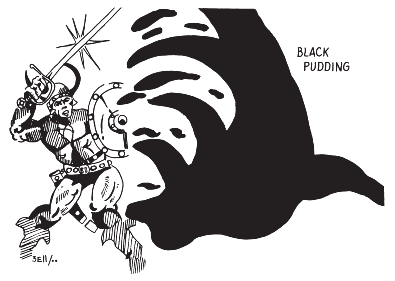
\includegraphics[width=0.8\linewidth]{./images/black-pudding.png}
\end{center}

%- - - - - - - - - - - - - - - - - - - - - - - - - - - SUB SUB SECTION
\phantomsection\subsubsection*{Dommages causés par type d'armes :}
\addcontentsline{toc}{subsubsection}{Dommages causés par type d'armes}

Si le système de dommage variables par type d'armes est utilisé, les divers monstres devront aussi être sujets à recevoir des points de dommages additionnels ou des dés de dommages. (Voir \textbf{Attaques et dommages par type de monstre}).

\bigskip

\begin{tabular}{lccc}
\textit{Type d'armes} & \textit{contre-} & \textit{-Opposants taille humaine-} & \textit{-Opposants plus grands-} \\
Dague                          && 1--4 points  & 1--3 points \\
Hache à main                   && 1--6 points  & 1--4 points \\
Masse, piolet*, marteau de nain && 1--6 points  & 1--4 points \\
Epée                           && 1--8 points  & 1--12 points \\
Hache de bataille*             && 1--8 points  & 1--8 points \\
Masse à pointes**              && 1--8 points  & 1--6 points \\
Fléau d'armes ***              && 1--8 points  & 1--8 points \\
Lance, lancée/enfoncée         && 1--6 points  & 1--8 points \\
Lance, enfoncée contre charge  && 1--8 points  & 2--12 points \\
Lance, posée contre charge     && 1--10 points & 2--16 points \\
Armes d'hast****               && 1--8 points  & 1--12 points \\
Hallebarde***                  && 1--10 points & 2--12 points \\
Epée à deux mains***           && 1--10 points & 3--18 points \\
Lance de tournoi               && 1--8 points  & 2--24 points \\
Pique****                      && 1--8 points  & 1--12 points \\
Flèche ou carreau              && 1--6 points  & 1--6 points \\
Pierre de fronde               && 1--4 points  & 1--6 points \\
\end{tabular}

\begin{tabular}{rp{15cm}}
\multicolumn{1}{r}{*} & l'arme requiert au moins 1.2m d'espace de chaque côté du porteur \\
\multicolumn{1}{r}{**} & l'arme requiert au moins 1.5m d'espace de chaque côté du porteur \\
\end{tabular}

\begin{tabular}{rp{15cm}}
\multicolumn{1}{r}{***} & l'arme requiert au moins 1.8m d'espace de chaque côté du porteur \\
\multicolumn{1}{r}{****} & la règle générale est que ces armes ne sont pas utilisables dans les donjons en raison de leur longueur \\
\end{tabular}

%- - - - - - - - - - - - - - - - - - - - - - - - - - - SUB SUB SECTION
\phantomsection\subsubsection*{Attaques et dommages par type de monstre}
\addcontentsline{toc}{subsubsection}{Attaques et dommages par type de monstre}

Ce système doit être utilisé avec les dommages variables par arme et, en aucun cas, il n'est recommandé de l'utiliser sans la mécanique susmentionnée.

\bigskip

\begin{tabular}{p{4cm}>{\raggedright\arraybackslash}p{5cm}>{\raggedright\arraybackslash}p{6.5cm}}
\textit{Type de monstre} && \textit{Points de dommages} \\
\hspace{0.5cm}\textit{attaquant} & \textit{Nombre d'attaques} & \hspace{0.5cm}\textit{par attaque} \\
Homme & 1 ou 2 & Dépend du type d'arme \\
Gobelin/Kobold & 1 & 1--4 ou par type d'arme \\
Orc & 1 & 1--6 ou par type d'arme \\
Hobgobelin/Gnoll & 1 & 1--8 ou par type d'arme \\
Ogre  & 1 & 1--10 \\
Troll & 2 griffes/1 morsure & 1--4/griffe, 1--8/morsure \\
Géant & 1 & COLLINE --- 2--16 \\
&& PIERRE --- 3--18 \\
&& GIVRE --- 4--24 \\
&& FEU --- 5--30 \\
&& NUAGE --- 6--36 \\
Squelette & 1 & 1--6 \\
Zombie & 1 & 1--8 \\
Goule & 2 griffes/1 morsure & 1--3/griffe, 1--4/morsure \\
Wight & 1 & Drain d'énergie seulement \\
Wraith & 1 & 1--6 et drain d'énergie \\
Momie & 1 & 1--12 \\
Spectre & 1 & 1--8 et drain d'énergie \\
Vampire & 1 & 1--10 et drain d'énergie \\
Cocatrix & 1 & 1--6 et changement en pierre \\
Basilic & 1 & 1--10 et changement en pierre \\
Méduse & 1 ou 2 & par type d'arme et changement en pierre \\
Gorgone* & 1 coup & 2--12/coup \\
Manticore & 2 griffes/1 morsure/24 pics & 1--3/griffe, 1--8/morsure, 1--6/pic \\
Hydre & 1 par tête & 1--6, 1--8, 1--10 selon la taille \\
Chimère & 2 griffes/3 têtes & 1--3/griffe ;\\
&& TETE DE CHEVRE --- 1--4/corne \\
&& TETE DE LION --- 1--8/morsure \\
&& TETE DE DRAGON --- 3-12/morsure** \\
Wyverne & 1 morsure/1 dard & 2-16/morsure, 1-6/dard*** \\
\end{tabular}


\begin{tabular}{p{4cm}>{\raggedright\arraybackslash}p{5cm}>{\raggedright\arraybackslash}p{6.5cm}}
\textit{Type de monstre} && \textit{Points de dommages} \\
\hspace{0.5cm}\textit{attaquant} & \textit{Nombre d'attaques} & \hspace{0.5cm}\textit{par attaque} \\
Dragon* & 2 griffes/1 morsure & 1--4/griffe ; \\
&& BLANC --- 2--16/morsure \\
&& NOIR --- 3--18/morsure \\
&& VERT --- 2--20/morsure \\
&& BLEU --- 2--24/morsure \\
&& ROUGE --- 3--30/morsure \\
&& DORE --- 3--36/morsure \\
Gargouille & 2 griffes/1 morsure/1 corne & 1--3/griffe, 1--6/morsure, 1--4/corne \\
Lycanthrope & LOUP --- 1 morsure & 2--8/morsure \\
& SANGLIER --- 1 morsure & 2--12/morsure \\
& TIGRE --- 2 griffes/1 morsure & 1--4/griffe, 1--10/morsure \\
& OURS --- 2 griffes/1 morsure & 1--3/griffe****, 2--8/morsure \\
Vert pourpre & 1 morsure/1 piqûre & 2-24/morsure, 1-8/piqûre*** \\
Monstre marin & 1/tête ou /tentacule ou par griffe & entre 3--24 et 5--50/tête, ou 2--12 et 4--24/tentacule ou 2--8 et 4--32/griffe \\
Minotaure & 1 coup/1 morsure/1 arme & 2--8/coup, 1--3/morsure, par type d'arme \\
Centaure & 2 sabots/1 arme & 1--6/sabot, par type d'arme \\
Licorne & 2 sabots/1 corne & 1--8/sabot, 1-16/corne \\
Nixe & 1 & 1--4 ou par type d'arme \\
Dryade & 1 & 1--4 ou par type d'arme \\
Gnome & 1 & 1--6 ou par type d'arme \\
Nain & 1 & 1--8 ou par type d'arme \\
Elfe & 1 & 1--10 ou par type d'arme \\
Ent & 2 & 2--16, 3--18, ou 4--24/attaque selon taille \\
Pégase & 2 sabots & 1--8/sabot \\
Hippogriffe & 2 griffes/1 morsure & 1--6/griffe, 1--10/morsure \\
Rokh & 2 griffes/1 morsure & 1--8, 2--12 ou 4--16/griffe, 2--12, 3--18 ou 4--24/morsure selon taille \\
Griffon & 2 griffes/1 morsure & 1--4/griffe, 2--16/morsure \\
Harceleur invisible & 1 & 4--16 \\
Elémentaire***** & 1 & AIR --- 2--16 \\
&& TERRE --- 4--32 \\
&& FEU --- 3--24 \\
&& EAU --- 3--30 \\
Djinn & 1 & 2--16 \\
Efrit & 1 & 3--24 \\
Gelée ocre & 1 & 2--12 \\
Black Pudding & 1 & 3--24 \\
Slime vert & 1 & spécial \\
Vase grise & 1 & 2--16 \\
\end{tabular}

\begin{tabular}{p{4cm}>{\raggedright\arraybackslash}p{5cm}>{\raggedright\arraybackslash}p{6.5cm}}
\textit{Type de monstre} && \textit{Points de dommages} \\
\hspace{0.5cm}\textit{attaquant} & \textit{Nombre d'attaques} & \hspace{0.5cm}\textit{par attaque} \\
Moisissure jaune & 1 & spécial \\
Petit cheval & 2 sabots & 1--4/sabot \\
Cheval moyen & 2 sabots/1 morsure & 1--6/sabot, 1-3/morsure \\
Grand cheval & 2 sabots/1 morsure & 1--8/sabot, 1-3/morsure \\
Rat géant (de Sumatra) & 1 morsure & 1-3/morsure \\
Loup & 1 morsure & 1-6/morsure \\
Canis Dirus & 1 morsure & 1-8/morsure \\
Lion & 2 griffes/1 morsure & 1--3/griffe, 1--10/morsure \\
Tigre à dents de sabre & 2 griffes/1 morsure & 1--4/griffe, 2--12/morsure \\
Belette géante & 1 morsure & 2--8/morsure plus drain de sang \\
Mammouth & 2 défenses/1 tronc/2 pieds & 3--18/défense, 2--16/tronc,
2--12/pied \\
Araignée géante & 1 morsure & 1--3*** plus toiles \\
Lézard géant & 1 morsure & 1--8/morsure \\
Crapaud géant & 1 morsure & 1--10/morsure \\
Serpent géant & 1 morsure, une constriction & 1--6/morsure***, 2--8/tour de constriction \\
Crabe géant & 2 pinces & 2--12/pince \\
Scarabée géant & 1 morsure & 3--30/morsure \\
Scorpion géant & 2 pinces/1 dard & 1--10/pince, 1--4***/dard \\
Crocodile & 1 morsure & 3--12/morsure \\
Tyrannosaurus rex & 1 morsure & 5--40/morsure \\
Triton & 1 & 3--18 plus spécial \\
Bugbear & 1 & 2--8 \\
Ogre mage & 1 & 1--12 \\
Géant, ORAGE & 1 & 7--42 \\
Titan & 1 & 7--42 \\
Ombre & 1 & 1--4 plus spécial \\
Feu follet & spécial & spécial \\
Liche & 1 & 1--10 plus spécial \\
Harpie & 2 griffes/1 arme & 1--3/griffe, 1--6/arme \\
Homme-lézard & 2 griffes/1 morsure & 1--3/griffe, 1--8/morsure \\
Doppleganger & 1 & 1--12 plus spécial \\
Dragon & 2 griffes/1 morsure & 1--4/griffe \\
&& AIRAIN --- 4--16/morsure \\
&& CUIVRE --- 5--20/morsure \\
&& BRONZE --- 3--24/morsure \\
&& ARGENT --- 3-30/morsure \\
Lycanthrope : Rat-garou ou homme-rat & 1 morsure/1 arme & 1--3/morsure, par type d'arme \\
Lammasu & 2 griffes & 1--6/griffe plus spécial \\
\end{tabular}

\begin{tabular}{p{4cm}>{\raggedright\arraybackslash}p{5cm}>{\raggedright\arraybackslash}p{6.5cm}}
\textit{Type de monstre} && \textit{Points de dommages} \\
\hspace{0.5cm}\textit{attaquant} & \textit{Nombre d'attaques} & \hspace{0.5cm}\textit{par attaque} \\
Salamandre***** & 1 touché/1 constriction/1 arme & spécial, 2--8/tour de constriction, par type d'arme \\
Beholder & 1 morsure & 2--5 plus spécial \\
Mastodonte des ombres & 2 griffes/1 morsure & 1--12/griffe, 2--8/morsure \\
Bête éclipsante & 2 tentacules & 2--8/tentacule \\
Chien esquiveur & 1 morsure & 1--6/morsure \\
Chien de chasse infernal* & 1 morsure & 1--6/morsure \\
Araignée de phase & 1 morsure & 1--6/morsure*** \\
Oxydeur & 1 toucher & spécial \\
Stirge & 1 morsure & 1--3 plus draine le sang \\
Tique géante & 1 morsure & 1--4 plus draine le sang \\
Ours-Hiboux & 2 griffes/1 morsure & 1--6/griffe****, 2--12/morsure \\
Charognard rampant & 8 tentacules & spécial \\
Cube gélatineux & 1 & 2--8 spécial \\
Limace géante & 1 morsure & 1--12 plus spécial \\
Homoncule & 1 morsure & 1--3 plus spécial \\
Golem & 1 & CHAIR --- 2--16 \\
&& PIERRE --- 3--24 \\
&& FER --- 4--32 \\
\end{tabular}
\begin{tabular}{rp{14.5cm}}
\multicolumn{1}{r}{*} & possèdent aussi leur souffle comme arme \\
\multicolumn{1}{r}{**} & à moins que le souffle soit utilisé \\
\multicolumn{1}{r}{***} & quelque soit le résultat, jet de sauvegarde contre le poison \\
\multicolumn{1}{r}{****} & une étreinte avec un score de 18 ou plus cause 2--16 points de dommages supplémentaires \\
\multicolumn{1}{r}{*****} & voir les différentes sections concernant tous les types d'élémentaires car des ajustements pourraient être requis en raison des circonstances
\end{tabular}

%----------------------------------------------------- SUB SECTION
\phantomsection\subsection*{EXPLICATION DES SORTS :}
\addcontentsline{toc}{subsection}{EXPLICATION DES SORTS}

%- - - - - - - - - - - - - - - - - - - - - - - - - - - SUB SUB SECTION
\phantomsection\subsubsection*{\textit{Magiciens :}}
\addcontentsline{toc}{subsubsection}{Magiciens}

\textit{Troisième niveau :}

\bigskip

\label{sort-suggestion}\textbf{Suggestion} : un sort qui fonctionne que le principe de l'hypnose. Si une créature sur laquelle le sort est lancé rate son jet de sauvegarde contre la magie, elle sera la victime de la suggestion, immédiatement ou de manière différée au bon vouloir du magicien. Le fait que la créature s'autodétruise est improbable à 99\%, mais des suggestions formulées avec attention peuvent, selon l'estimation de l'arbitre, altérer cette probabilité. Les suggestions doivent être simples et relativement courtes, soit une phrase ou deux. Durée : une semaine de temps de jeu.

\bigskip

\textit{Neuvième niveau :}

\bigskip

\label{sort-astral}\textbf{Sort astral} : un sort qui permet à l'utilisateur d'envoyer sa forme astrale, indétectable pour tous sauf pour ceux du plan astral, depuis son corps vers d'autres endroits. Noter qu'un sort ``Mot de pouvoir aveuglant'' ne pourrait pas empêcher ce sort et ne pourrait pas aveugler la forme astrale. Le magicien peut utiliser des sorts quand il est dans sa forme astrale, mais il y a 5\% de risques par niveau de sort que le sort échoue. Si le sort échoue, il y a un risque de 2\% par niveau de sort que le magicien soit forcé de retourner dans son corps. Exemple : un magicien du dix-huitième niveau dans sa forme astrale tente de jeter un sort du sixième niveau. Il y  30\% de chances que le sort échoue, et s'il échoue, il y a 12\% de chances qu'il soit obligé de réintégrer son corps. Si, pendant que le magicien a quitté son corps et se trouve dans le plan astral, son corps est bougé en dehors de la porté du sort ou détruit, la forme astrale du magicien est immédiatement envoyée pour bafouiller et hurler au plus bas niveau de l'enfer. Durée : dans les souterrains -- 12 tours ; à l'extérieur -- 8 heures de jeu. Portée : dans les souterrains -- 7m ; à l'extérieur -- 160km/niveau à partir du 18\textsuperscript{ème}. Mouvement du corps astral : dans les souterrains -- 4m/tour ; à l'extérieur 160km par heure de jeu depuis le 18\textsuperscript{ème} niveau.


%==========================================================================SECTION
\newpage
\phantomsection\section*{Monstres \& Trésors}
\addcontentsline{toc}{subsection}{Monstres \& Trésors}

\begin{center}
\textbf{[SELECTION]}
\end{center}

%----------------------------------------------------- SUB SECTION
\phantomsection\subsection*{EXPLICATIONS DES OBJETS MAGIQUES}
\addcontentsline{toc}{subsection}{EXPLICATIONS DES OBJETS MAGIQUES}

%- - - - - - - - - - - - - - - - - - - - - - - - - - - SUB SUB SECTION
\phantomsection\subsubsection*{POTIONS :}
\addcontentsline{toc}{subsubsection}{POTIONS}

\label{objet-huile-etheree}\textit{Huile éthérée} : quand l'utilisateur est oint de cette substance, il est capable de traverser des substance solides comme il le souhaite, comme s'il revêtait l'Armure Ethérée. Noter que quand l'utilisateur est ainsi oint, il n'est pas capable de manipuler des objets normaux car ses mains leur passent au travers.
